\documentclass[a4paper,UKenglish,cleveref, autoref, cleveref, thm-restate,pdfa]{lipics-v2021}
%for section-numbered lemmas etc., use "numberwithinsect"
%for enabling cleveref support, use "cleveref"
%for enabling autoref support, use "autoref"
%for anonymousing the authors (e.g. for double-blind review), add "anonymous"

%\graphicspath{{./graphics/}}%helpful if your graphic files are in another directory

\bibliographystyle{plainurl}% the mandatory bibstyle

\title{Towards better explanations for Constraint Satisfaction and Optimisation problems} %TODO Please add

\titlerunning{Towards better explanations for CSPs and COPs} %TODO optional, please use if title is longer than one line

\author{Emilio Gamba}{Data Analytics Lab - DTAI, VUB - KU Leuven, Belgium}{emilio.gamba@vub.be}{[0000-0003-1720-9428]}{}

\authorrunning{E. Gamba} 
%\authorrunning{J.\,Q. Public and J.\,R. Public} %TODO mandatory. First: Use abbreviated first/middle names. Second (only in severe cases): Use first author plus 'et al.'

\Copyright{CC-BY} %TODO mandatory, please use full first names. LIPIcs license is "CC-BY";  http://creativecommons.org/licenses/by/3.0/


\ccsdesc[500]{Theory of computation~Constraint and logic programming}

\keywords{Explainability, Unsatisfiable Subset Optimization, Constraint Satisfaction and Optimization problems} %TODO mandatory; please add comma-separated list of keywords

%\category{} %optional, e.g. invited paper

\relatedversion{} %optional, e.g. full version hosted on arXiv, HAL, or other respository/website
%\relatedversiondetails[linktext={opt. text shown instead of the URL}, cite=DBLP:books/mk/GrayR93]{Classification (e.g. Full Version, Extended Version, Previous Version}{URL to related version} %linktext and cite are optional

%\supplement{}%optional, e.g. related research data, source code, ... hosted on a repository like zenodo, figshare, GitHub, ...
%\supplementdetails[linktext={opt. text shown instead of the URL}, cite=DBLP:books/mk/GrayR93, subcategory={Description, Subcategory}, swhid={Software Heritage Identifier}]{General Classification (e.g. Software, Dataset, Model, ...)}{URL to related version} %linktext, cite, and subcategory are optional

%\funding{(Optional) general funding statement \dots}%optional, to capture a funding statement, which applies to all authors. Please enter author specific funding statements as fifth argument of the \author macro.

\acknowledgements{This research received partial funding from the Flemish Government (AI Research Program); and funding from the European Research Council (ERC) under the European Union’s Horizon 2020 research and innovation program (Grant No. 101002802, CHAT-Opt).}%optional

%\nolinenumbers %uncomment to disable line numbering

\hideLIPIcs  %uncomment to remove references to LIPIcs series (logo, DOI, ...), e.g. when preparing a pre-final version to be uploaded to arXiv or another public repository

%Editor-only macros:: begin (do not touch as author)%%%%%%%%%%%%%%%%%%%%%%%%%%%%%%%%%%
\EventEditors{John Q. Open and Joan R. Access}
\EventNoEds{2}
\EventLongTitle{42nd Conference on Very Important Topics (CVIT 2016)}
\EventShortTitle{CVIT 2016}
\EventAcronym{CVIT}
\EventYear{2016}
\EventDate{December 24--27, 2016}
\EventLocation{Little Whinging, United Kingdom}
\EventLogo{}
\SeriesVolume{42}
\ArticleNo{23}
%%%%%%%%%%%%%%%%%%%%%%%%%%%%%%%%%%%%%%%%%%%%%%%%%%%%%%

\usepackage[usenames,dvipsnames]{xcolor}
\usepackage{amsmath,amssymb,amsthm}
\usepackage[ruled,linesnumbered]{algorithm2e}
\usepackage{thmtools} 
\usepackage{booktabs}
\usepackage{paralist}
\usepackage{caption}
\usepackage{subcaption}
\usepackage{graphicx}
\usepackage{adjustbox}
\usepackage{multirow,array}
\usepackage{lscape}
\usepackage{tabularx}
\usepackage{enumitem}
\usepackage[capitalise]{cleveref}

\usepackage{cancel}
\usepackage{makecell}
\usepackage{cellspace}

\setlength\cellspacetoplimit{4pt}
\setlength\cellspacebottomlimit{4pt}
\addparagraphcolumntypes{X}

%%%%%%

\newlist{RQ}{enumerate}{1}
\setlist[RQ]{label=\bfseries{}RQ\arabic*:}
\newlist{WP}{enumerate}{1}
\setlist[WP]{label=\bfseries{}RQ\arabic*:}

\newcommand\m[1]{\mathcal{#1}}

\newtheorem{prob}{Problem}
\newtheorem{problem}[prob]{Problem Statement}


%% Comments
\newcommand\commentmargin[1]{\marginpar{\tiny #1}}
%\renewcommand\comment[1]{#1}
%\renewcommand\commentmargin[1]{}
\newcommand{\tias}[1]{{\commentmargin{\color{blue}Tias:#1}}}
\newcommand{\emilio}[1]{{\commentmargin{\color{red}Emilio: #1}}}
\newcommand{\checkthis}[1]{{\commentmargin{\color{red}CheckRephrasing: #1}}}
\newcommand{\bart}[1]{{\commentmargin{\color{OliveGreen}Bart: #1}}}
\newcommand{\new}[1]{{\commentmargin{{\color{blue} #1}}}}
\newcommand{\removed}[1]{\sout{#1}}

%% Factoring

\newcommand\call[1]{\mm{\texttt{#1}}}
\newcommand\mm[1]{\ensuremath{#1}\xspace}


\newcommand{\algorithmicbreak}{\textbf{break}}

%%%%%
%%%%%%
\usepackage[usenames,dvipsnames]{xcolor}
\usepackage{xspace}

% \newcommand\advice[2][]{\par {\color{OliveGreen} \textsc{ADVICE:} #1} \par} 

\def \ifempty#1{\def\temp{#1} \ifx\temp\empty }

\usepackage{xparse}

\NewDocumentCommand{\advice}{om}{%
\par {\color{OliveGreen} \textsc{ADVICE:} #2  
\ifempty{#1} {} \else {\bf In this case: #1} \fi 
} \par
}



%%%%%%%%%%%%%%%%%%%%%%%%
% GIT
%%%%%%%%%%%%%%%%%%%%%%%%
\newcommand{\TIPnoartefactsingit}[1][]{\advice[#1]{Do not add files produced by latex (aux, pdf, log, ...) to your git repository. If for some reason, you wish to include a pdf in your git repo, e.g., for archival reasons, give it another name, e.g., ``version-submitted-to-ICLP21.pdf''}}
\newcommand{\TIPnoforcedpushes}[1][]{\advice[#1]{Never use forced pushes in git}}
\newcommand{\TIPgitmergetool}[1][]{\advice[#1]{p4merge is an excellent merge tool for git. Solves lots of your problems}}
\newcommand{\TIPglobalgitignore}[1][]{\advice[#1]{You can make a global gitignore file. So that you don't have to ignore them in each repository: \url{https://gist.github.com/subfuzion/db7f57fff2fb6998a16c}, e.g., with ``git config --global core.excludesFile 'path_to_global_gitignore_file'''}} 


%%%%%%%%%%%%%%%%%%%%%%%%
% LaTeX + GIT
%%%%%%%%%%%%%%%%%%%%%%%%
\newcommand{\TIPonelinesentence}[1][]{\advice[#1]{When using git with LaTeX, in my experience, the best way to go is:
\begin{itemize}
 \item Put a newline after every sentence
 \item Disable any forms of (hard) line wrapping in your editor
\end{itemize}
The reason for this is the way git handles conflicts. Git will detect a conflict when two lines close to each other change. 
When viewing this from a LaTeX perspective: changes in a sentence are probably only related to the sentences close to it. 
Hard line wrapping is terrible in this respect. 
}}



%%%%%%%%%%%%%%%%%%%%%%%%
% CITATIONS 
%%%%%%%%%%%%%%%%%%%%%%%%
\newcommand{\TIPspacebeforecite}[1][]{\advice[#1]{Do not let your citations stick to the previous word. Leave a space before it, as in ``he did this \cite{something}'' or ``he did this~\cite{something}'', the latter in case you do not want a line break to happen between the sentence and the citation (often, this is best)}}
\newcommand{\TIPcitemultiple}[1][]{\advice[#1]{When citing multiple papers, use \cite{one,two}, not \cite{one}\cite{two}}}
\newcommand{\TIPcitet}[1][]{\advice[#1]{In general, I prefer the practice where everything between brackets can be dropped and still yield a sentence. 
This also means: do not use citations as objects. Do not say: 
``(Bogaerts 2021) showed that \dots'' or ``[1] showed that \dots'', but write ``Bogaerts (2018) showed that \dots'' or ``Bogaerts [1] showed that \dots''. 
Depending on your latex styles and citation styles, you can use \texttt{$\backslash$citet} (or \texttt{citeauthor} or ...) to get this for free}}
\newcommand{\TIPcitetINperson}[1][]{\advice[#1]{When using \texttt{$\backslash$citet}, make sure to get your prepositions right. Author-names refer to persons. Not a lot has been done ``in Bogaerts'', so never write ``in \texttt{$\backslash$citet$\{\dots\}$}'', but ``by  \texttt{$\backslash$citet$\{\dots\}$}''.}}
\newcommand{\TIPcitetDoNotOveruse}[1][]{\advice[#1]{While it is good to use commands such as \texttt{$\backslash$citet}, do not overuse them. For instance do not write ``it is well-known that $P$ according to \citet{X}''. Instead simply write: ``it is well-known that $P$ \cite{X}'' (or \texttt{pcite} or ... (depending on the style/packages used)). The property ``everything between brackets can be dropped and we still ahve a sentence'' is still satisfied}}
\newcommand{\TIPcitetAuthorCount}[1][]{\advice[#1]{When using commands such as \texttt{$\backslash$citet}, mind your author count: ``\citet{X} proposes that'' (single author) vs ``\citet{X} propose that'' (but in this case, past tense might be better).}}
\newcommand{\TIPreferenceInSentence}[1][]{\advice[#1]{Put your references in the sentence not after. ``This is good \cite{}.'' ``This is not good. \cite{}''}}


%%%%%%%%%%%%%%%%%%%%%%%%
% TEXT
%%%%%%%%%%%%%%%%%%%%%%%%
\newcommand{\TIPusequotes}[1][]{\advice[#1]{Use the right quotes: Never use "this is a quote", but always ``this is a quote''}}
\newcommand{\TIPspacingafterabbreviation}[1][]{\advice[#1]{After a full stop, LaTeX leaves more than the standard spacing. If the dot comes from an abbreviation, you should take care of getting back normal spacing: write ``pigeons (resp.\ holes)'' and not ``pigeons (resp. holes)''. }}
\newcommand{\TIPspacingOrCommaAfterIEorEG}[1][]{\advice[#1]{After a full stop, LaTeX leaves more than the standard spacing. When this is not desired, some manual fix is needed. In the case of ``i.e.'' and ``e.g.'', there are two options: either write ``i.e.\ something'' or write ``i.e., something'' (I prefer the comma variant). }}
\newcommand{\TIPemphasizeDefinedConcept}[1][]{\advice[#1]{Emphasize every concept you define, e.g., a \emph{literal} is an atom $x$ or its negation $\neg x$}}


%%%%%%%%%%%%%%%%%%%%%%%%
% SPACING
%%%%%%%%%%%%%%%%%%%%%%%%
%TODO  Do not put {} around text. Example.

%%%%%%%%%%%%%%%%%%%%%%%%
% DASHES
%%%%%%%%%%%%%%%%%%%%%%%%
\newcommand{\TIPrangeEnDash}{For (page) ranges, use an En-dash: write: 1--10 instead of 1-10.}

%%%%%%%%%%%%%%%%%%%%%%%%
% MATH MODE
%%%%%%%%%%%%%%%%%%%%%%%%

\newcommand{\TIPnonamesinmathmode}[1][]{\advice[#1]{Do not use names of things longer than one character in math mode. By this I mean: do not write 
\[ force = mass \cdot acceleration\]
because this looks HORRIBLE. The formattig Latex applies is as if you want 
\[f\cdot o\cdot r \cdot c \cdot e = \dots\]
What you should do is: 
\[ \mathit{force} = \mathit{mass}\cdot \mathit{acceleration}\]
(or mathrm depending on what you like). 
Of course... even better: do not repeat this mathit all over your document, but make a command out of it!} }
\newcommand{\TIPmathit}[1][]{\TIPnonamesinmathmode[#1]}
\newcommand{\TIPmathalwaysindollars}[1][]{\advice[#1]{\textbf{Always} write your math in a math environment. \textbf{Never} mimick it, e.g., by using \textit{k} in text instead of $k$, even if you think it looks similar. It might look very different in another style (and also things like $k-1$ are not the same as \textit{k-1})}}
\newcommand{\TIPstrictNonstrictInclusion}[1][]{\advice[#1]{I prefer to only use $\subseteq$ and $\subsetneq$ since $\subset$ is ambiguous (depending on which book you use it means strict or non-strict inclusion}}
\newcommand{\TIPspacingOfOperators}[1][]{\advice[#1]{Be careful when using an operator as an ``object''. For instance if you say $\bowtie\in\{\leq, \geq\}$ notice that the spacing is off (compare to $x\in \{y,z\}$). You can trick LaTeX into thinking that bowtie is not an operator in this formula as follows:  ${\bowtie}\in\{\leq, \geq\}$.}}
\newcommand{\TIPdoubledollar}[1][]{\advice[#1]{Never use double dollars for math displays. See \url{https://tex.stackexchange.com/questions/503/why-is-preferable-to}}}

%%%%%%%%%%%%%%%%%%%%%%%%
% CAPITALS  
%%%%%%%%%%%%%%%%%%%%%%%%
\newcommand{\TIPcapitalboolean}[1][]{\advice[#1]{I prefer Boolean to be written with a capital letter (refers to George Boole). But some people use lowercase}}
\newcommand{\TIPcapitalTitles}[1][]{\advice[#1]{Use consistent capitalization of section titles. Either always ``every'' word capitalized, or always only the first word... It might be that the venue (conference/journal) has guidelines about this}}


%%%%%%%%%%%%%%%%%%%%%%%%
% FORMATTING
%%%%%%%%%%%%%%%%%%%%%%%%
\newsavebox\VerbTIPcommandforconsistentformatting
\begin{lrbox}{\VerbTIPcommandforconsistentformatting}
\begin{minipage}{\textwidth}
\begin{verbatim}
\newcommand\uriname[1]{\texttt{#1}\xspace}
\end{verbatim}
\end{minipage}
\end{lrbox}
\newcommand{\TIPcommandforconsistentformatting}[1][]{\advice[#1]{If your paper contains a lot of objects that have to be formatted in a similar way, e.g., lots of symbols for Boolean variables, or lots of URIs (in a semantic web context), make a command for this, to easily allow changing the formatting later, e.g., as follows:}
\usebox{\VerbTIPcommandforconsistentformatting}
}

%%%%%%%%%%%%%%%%%%%%%%%%
% NAMES & Symbols 
%%%%%%%%%%%%%%%%%%%%%%%%



%%%%%%%%%%%%%%%%%%%%%%%%
% DEFINITIONS  (MACROS)
%%%%%%%%%%%%%%%%%%%%%%%%
\newsavebox\VerbTIPnobracketsarounddefinitionsWRONG
\begin{lrbox}{\VerbTIPnobracketsarounddefinitionsWRONG}
\begin{minipage}{\textwidth}
\begin{verbatim}
 \newcommand{\leqp}{{\leq_p}}
 \end{verbatim}
\end{minipage}
\end{lrbox}
\newsavebox\VerbTIPnobracketsarounddefinitionsRIGHT
\begin{lrbox}{\VerbTIPnobracketsarounddefinitionsRIGHT}
\begin{minipage}{\textwidth}
\begin{verbatim}
 \newcommand{\leqp}{\leq_p}
\end{verbatim}
\end{minipage}
\end{lrbox}
\newcommand{\TIPnobracketsarounddefinitions}[1][]{\advice[#1]{When defining a command, do not put the thing you defin in between brackets, i.e., do not write
 \usebox{\VerbTIPnobracketsarounddefinitionsWRONG}
but write
 \usebox{\VerbTIPnobracketsarounddefinitionsRIGHT}
The reason is: these brackets mess up spacing}}

\newcommand{\TIPmakeMacroForConcepts}[1][]{
\advice[#1]{If you have an often-occurring concept, make a macro for it. For instance: do not write, ``Let $\Sigma$ be a set of Boolean variables'' but make a command, e.g. $\\$\texttt{voc} for a ``vocabulary''. That way, if it turns out later that you have used $\Sigma$ for two different things, you can easily replace it}}

\newcommand{\TIPconsistentNames}[1][]{
\advice[#1]{Try to use consistent names for the same symbols. Do not call interpretations $I$ and later $J$ (unless you need to distsinguish between two interpretations)}}

%%%%%%%%%%%%%%%%%%%%%%%%
% WRITING
%%%%%%%%%%%%%%%%%%%%%%%%
\newcommand{\TIPavoidWeakVerbs}[1][]{\advice[#1]{Avoid writing weak verbs such as ``tries'' ``attempts to'', unless you really want to emphasize that this is an attempt, but probably not succesful. For instance when referring to other papers, do not write ``AUTHOR tries to solve the problem by \dots'' but write ``AUTHOR proposes an algorithm to \dots''. }}
\newcommand{\TIPnoContractions}[1][]{\advice[#1]{Avoid contractions such as ``it's'', ``isn't'', ``We'll'',... }} 


%%%%%%%%%%%%%%%%%%%%%%%%
% ENGLISH
%%%%%%%%%%%%%%%%%%%%%%%%
\newcommand{\TIPbothInEnglish}[1][]{\advice[#1]{In English, the sentence ``both x and y satisfy z'' mean ``x satisfies z and y satisfies z''. 
If you write for instance ``both conditions guarantee that ...'', you mean: ``just one of them suffices to guarantee that''. 
Also: writing things such as ``Both $x$ and $y$ are related'' does not really make sense. 
If you mean to say that $x$ is related to $y$, drop the ``both''.}}
\newcommand{\TIPcongruenceSubjectVerb}[1][]{\advice[#1]{Watch out for subject-verb congruence or verb-object congruence (plural vs singular). While not technically incorrect, sentences such as ```$x$ and $y$ are an important part of ...'' are sometimes hard to read. If both of them are an important part, this is wrong, but in some cases, such a sentence could be acceptable. However, even in such cases it is often possible to avoid the problem alltogether, here e.g., by writing ```$x$ and $y$ are imporant in...''.}}
\newcommand{\TIPLetThen}[1][]{\advice[#1]{I don't really like the construction ``Let x be a variable. Then [...]''. Some sources claim this is not gramatically correct, but... others accept it. In any case, I find it more clear if you can link your ```then''s with ``If''s. For instance instead of writing ```Let $x$ be a special  $A$ and $y$ a $B$. Then $x$ is greater than $y$.'', you can write ``Let $x$ be an $A$ and $y$ a $B$. If $x$ is special, then $x$ is greater than $y$.''}}


%%%%%%%%%%%%%%%%%%%%%%%%
% WRITING MATH 
%%%%%%%%%%%%%%%%%%%%%%%%
\newcommand{\TIPdefVSchoice}[1][]{\advice[#1]{Definitions should be deterministic. There is a big difference between ``Let $x$ be \textbf{a} [...]'' and ``Let $x$ be \textbf{the}''. The former cases chooses an $x$ with a certain property arbitrarily (this can be useful in case you wish to prove something to hold for all such $x$s). The second can be used to \emph{define} $x$ (uniquely)}}


%%%%%%%%%%%%%%%%%%%%%%%%
% 
%%%%%%%%%%%%%%%%%%%%%%%%


%%%%%%%%%%%%%%%%%%%%%%%%
% POINTERS
%%%%%%%%%%%%%%%%%%%%%%%%
% FOR MATHEMATICAL WRITING, SEE
% https://faculty.math.illinois.edu/~west/grammar.html#definitions
% 







%%%%%%% ALGORITHM KEYWORDS
\SetKwInOut{Input}{Input}
\SetKwInOut{OptInput}{Optional}
\SetKwInOut{Output}{Output}
\SetKwInOut{State}{State}
\SetKwInOut{Ext.}{Ext}
\SetKwComment{command}{/*}{*/}
\SetKw{Break}{break}
%%%%%%%

\renewcommand{\tabularxcolumn}[1]{m{#1}}%
\newcolumntype{C}{>{\centering\arraybackslash}X}

\begin{document}
\maketitle	

\begin{abstract}

\end{abstract}

	\section{Introduction}
	%\vspace*{2cm}	
	
	\subsection{Contributions}
	\begin{enumerate}
		\item We Correlation between explanation difficulty measured by cost-function and the perceived difficulty of a Sudoku
		\item We 
		\item We develop a method based on ....(Inverse Optimisation) for tuning the explanation to the user preferences 
	\end{enumerate}
	%\vspace*{2cm}	
	
	
	%	\section{Background}
	
	
	\section{Research questions}
	\begin{RQ}
		\item\label{Features-good-explanation} Which are the features of a good explanation?
		\begin{itemize}
			\item How do we encode the features of a good explanation in the cost-function?
			\item What are the limitations of current state-of-the-art for effectively computing explanations using OCUSs ?
		\end{itemize}
		\item \label{reconcicle-explanation-sequences} How to reconcile auto-generated sequences of explanations with human generated solving traces? 
		\begin{itemize}
		\item What are the global metrics  for characterizing the quality of an explanation sequence ?
		\item How do we capture the preferences of a user based on the features we have extracted for a good explanation?
%		\item How do we capture the preferences of a user based on the features we have extracted for a good explanation?
		\end{itemize}
		\item\label{meaningful-nested-sequence} Is it always possible to generate a meaningful nested explanation sequence ?
		\begin{itemize}
			\item Abstraction level
		\end{itemize}
	\end{RQ}
	
	\section{Research plan}
	
	\subsection{User-friendly explanations}
	
	
	\subsection{Preferred explanation sequences}
	
		
	\section{Explanations for Constraint Satisfaction and Optimization Problems}
	

	An explanation in the context of the Sudoku corresponds to a combination of constraints with a certain number of assignments in the interpretation. For instances in \cref{explanations:example} depicts two equivalent explanations for explaining why a 6 can be written at the puzzle piece. 
	
	\begin{figure}[!h]
		\begin{subfigure}{0.45\textwidth}\centering
			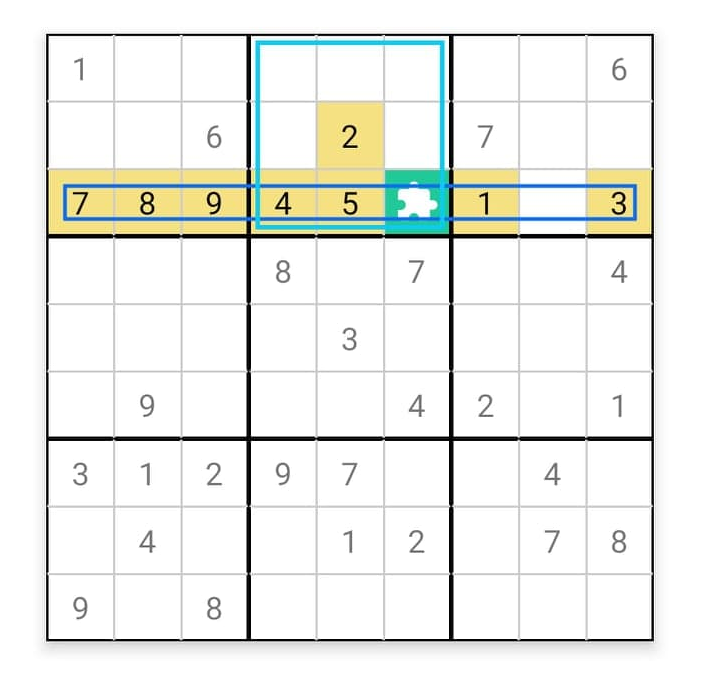
\includegraphics[width=0.8\textwidth]{figures/sudoku_hint_1.png}
			\caption{Using the highlighted digits, and all different values on row3, and all different values on block (1, 2), we can derive a 6 at the puzzle piece.}
			\label{alternative-explanation:same-block}
		\end{subfigure}\hfill
		\begin{subfigure}{0.45\textwidth}\centering
			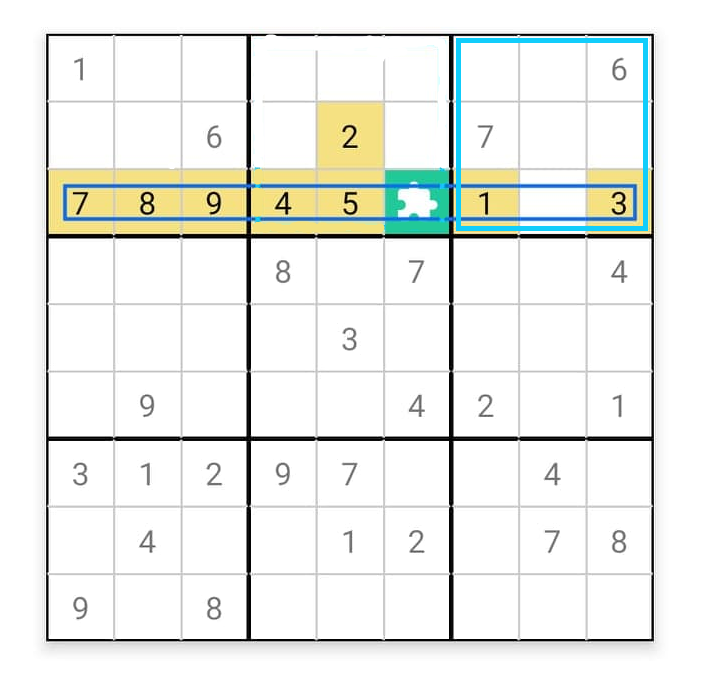
\includegraphics[width=0.8\textwidth]{figures/sudoku_hint_2.png}
			\caption{Using the highlighted digits, and all different values on row3, and 6 cannot be in block (1, 3), we can derive a 6 at the puzzle piece.}
			\label{alternative-explanation:other-block}
		\end{subfigure}
		\caption{Example of explanations for Sudoku.}
		\label{explanations:example}
	\end{figure}
	
		\begin{example}
		(Sudoku) The 9 x 9 Sudoku puzzle requires filling in numbers (1...9) in a grid, where the numbers can only appear: Once in every row \textbf{i} ($\mathbf{row_{i}}$);
		once in every column \textbf{j} ($\mathbf{col_{i}}$); and once every block \textbf{k} ([$\mathbf{block_{k}}$). The blocks of a given Sudoku are numbered starting from the top left to the bottom right. Typical solving processes use two types of notations: 
		\begin{itemize}
			\item $\mathbf{cell[1, 4] = 2}$ meaning  cell at row 1 and column 4 takes value 2;
			\item $\mathbf{cell[1, 4] \neq 7}$ meaning cell at row 1 and column 4 cannot take value 7 (domain reductions).
		\end{itemize}
	\end{example}
	
	
	\section{Features of a good explanation}
	
	\begin{itemize}
		\item Insights from the Social sciences by Tim Miller 
		\item Applciation to users
		\item Explanations in Constraint Satisfaction
		\item Use case of a SUdoku
	\end{itemize}		
	
	\subsection{Explanation quality} The quality of an explanation relates to the difficulty of understanding it. Therefore, the cognitive complexity of an explanation is approximated using a cost-function $f$. To the best of our knowledge there does not exist a good metric yet of what is and what is not a good cost function. Intuitively such a cost-function should at least take into account the type and the number of constraints and assignments in the interpretation.
	
	\begin{description}
		\item[baseline] We define the baseline cost-function as a weighted sum where the \texttt{row, block} and \texttt{col} constraints are assigned a weight of 20, and assignments have a unit weight.
		\item[Simon vandevelde's thesis\cite{master-thesis-sudoku}] use the following equation as a cost-function with $N$, the number of assignments, $R$ the number of rows constraints, $C$ the number of column constraints, $B$ the number of block constraints used in the explanation.
		\begin{equation}
			N \cdot (R + 1) \cdot (C + 1) \cdot (B + 1) 
		\end{equation} 
	\item[Other sources ??] See related works!
	\end{description}

	\subsection{Opportunities for improvement}
	The above mentioned cost-function do not take into account several elements worthy of improvement:
	\begin{description}
		\item[Temporality] Previously derived assignments:
		\begin{itemize}
			\item weighing scheme based on position in the explanation sequence it was derived in, i.e. previous step: 
			\[w_{\text{cell}[2, 3]} = 2 - \frac{1}{\text{\# step-derived}} \]
			\item ...
		\end{itemize}
		\item[Locality] Explain assignments that are `close' to each other
		\begin{description}
		\item[Sudoku-specific] User scans the Sudoku grid from Top-left to bottom right; and fills the numbers from 1 to 9.
		\end{description}
%		\item The cost of the explanation sequence
		\item[Nested explanation sequence] The length of the nested explanation sequence
	\end{description}

	
	\section{Explanation sequence}
	
	\subsection{Baseline}
	
	To compare potential improvements on the explanation sequence, we compute an explanation sequence where only assignments to the problem variables are considered. In this experiment, we focus on 2 elements: 
	\begin{inparaenum}
		\item The efficiency of generating a sequence
	\end{inparaenum}
	The following graphs present the cost and the time for generating an explanation sequence using calls to \texttt{split-OCUS}. 
	
	
	
	\begin{figure}[!h]
		\begin{subfigure}{0.45\textwidth}
		\centering
		\includegraphics[width=\textwidth]{figures/mean_cost_difficulty.pdf}
		\caption{Baseline: Max explanation cost of Sudoku instances}
		\label{fig:baseline:histogram:expl-cost}
		\end{subfigure}\hfill
		\begin{subfigure}{0.45\textwidth}
	\centering
	\includegraphics[width=\textwidth]{figures/max_cost_difficulty.pdf}
	\caption{Baseline: Max explanation cost of Sudoku instances}
	\label{fig:baseline:histogram:expl-cost}
\end{subfigure}\hfill
	\end{figure}
	
%	\todo{This is missing some results!}
	
	\subsection{Alternative explanations}
	
	\begin{problem}\label{problem-statement:alternative-explanations}
		At every explanation step, there potentially exist numerous alternative explanation steps of equal cost: 
		\begin{enumerate}
			\item Explanation steps where different combinations of constraints can be used to explain the same literal;
			\item Explanation steps of same cost that explain different literals.
		\end{enumerate}
	\end{problem}	
	
	\begin{figure}[!h]
		\begin{subfigure}{0.45\textwidth}\centering
			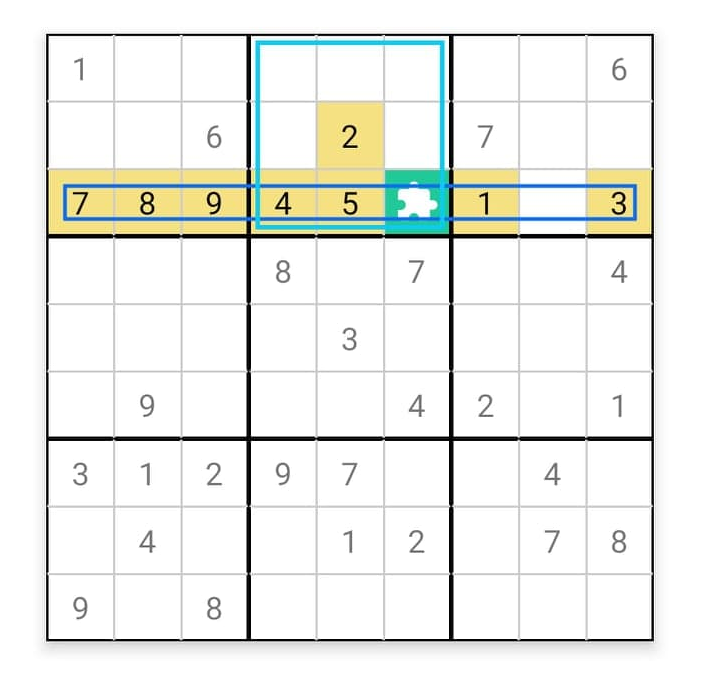
\includegraphics[width=0.8\textwidth]{figures/sudoku_hint_1.png}
			\caption{Using the highlighted digits, and all different values on row3, and all different values on block (1, 2), we can derive a 6 at the puzzle piece.}
			\label{alternative-explanation:same-block}
		\end{subfigure}\hfill
		\begin{subfigure}{0.45\textwidth}\centering
			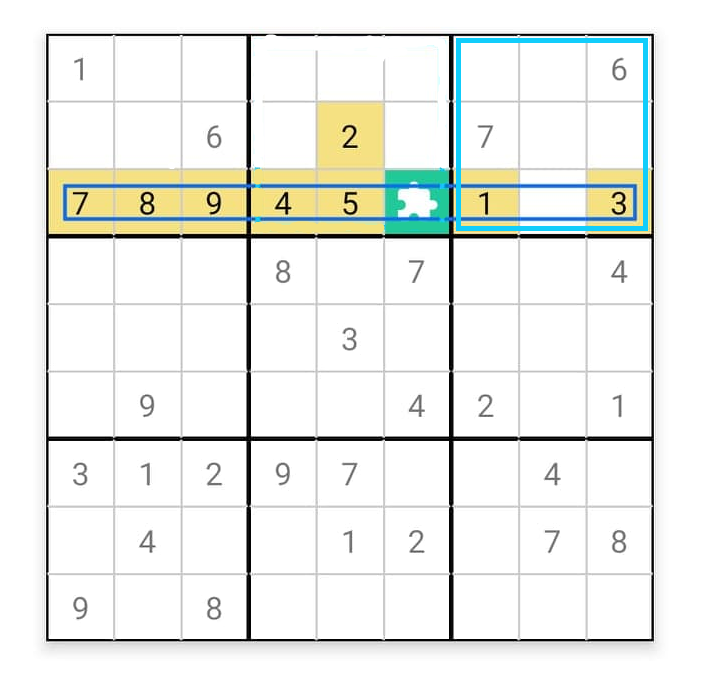
\includegraphics[width=0.8\textwidth]{figures/sudoku_hint_2.png}
			\caption{Using the highlighted digits, and all different values on row3, and 6 cannot be in block (1, 3), we can derive a 6 at the puzzle piece.}
			\label{alternative-explanation:other-block}
		\end{subfigure}
	\end{figure}
	
	
%	\subsection{Temporality of the explanations} 
%	\begin{problem}\label{problem-statement:locality-explanations}
%		One strategy to solve the Sudoku is to look at a specific number, for instance, the one that appear the most in the grid and try to fill in that same number in other blocks of the grid.
%	\end{problem}
	
	
	\subsection{Optimizing the sequence}
	\begin{problem}\label{problem-statement:sequence-optimisation}
		The sequence generation is greedily optimized.	At every explanation step of sequence, the cost-optimal explanation step is computed. However, there is \emph{no guarantee of optimality at the sequence level} with respect to a global metric.
	\end{problem}
	
	\begin{itemize}
		\item[Q1] What are the global metrics for quantifying the quality of an explanation sequence, i.e. optimizing the explanation sequence such that
		\begin{description}
			\item[Maximum] the cost of the most difficult explanation is as low as possible;
			\item[Average]  the average cost of the sequence is as low as possible.
		\end{description}	
	\end{itemize}	
	
	
	\subsection*{Naive and greedy approaches to improve explanation sequence}
	
	\begin{description}
		\item[Least-cost] Select least cost explanation step at every step of the sequence.
		\item[Breadth-first search] Explore the whole explanation search tree at least of O(n!) to find the least cost explanation sequence, where the cost of the explanation sequence can be used as a bound.
	\end{description}
	
	\section{Work Packages}
	
	\begin{WP}
		\item Features of a good explanation
		\item 		
	\end{WP}
	%TODO: Insert gantt chart here!
	
	\section{Experiments}
	
	The experiments are run on a laptop with a  2,6 GHz 6-Core Intel Core i7 processor, and 16 GB of RAM.
	The whole pipeline is implemented using CPMpy (\textit{write version here!}), with PySAT (\textit{write version here!}), as the default SAT solver, Gurobi (\textit{write version here!}) for the MIP solver. The benchmark instances consist of the Sudoku scanned by the Sudoku Assistant that have been corrected to make sure they are satisfiable and have a unique solution.
	
	
	\section{Experiments}
	
	\subsection{Research questions}
\begin{RQ}
	\item\label{Features-good-explanation} Which are the features of a good explanation?
	\begin{itemize}
		\item How do we encode the features of a good explanation in the cost-function?
	\end{itemize}
	\item \label{reconcicle-explanation-sequences} How to reconcile auto-generated sequences of explanations with human generated solving traces? 
	\begin{itemize}
		\item Which are the metrics  for characterizing the difficulty of an explanation sequence ?
		\item How do we learn the preferences of a user based on the features we have extracted for a good explanation?
	\end{itemize}
	\item\label{meaningful-nested-sequence} Is it always possible to generate a meaningful nested explanation sequence ?
\end{RQ}

	
	\newpage
	\begin{landscape}
		\section{Related Works}
		
		\begin{table}[!h]
			\begin{tabularx}{\linewidth}{|l|S{X}|S{X}|}
				\Xhline{1.5pt}
				Reference & Description (and properties) & Hint \\
				\Xhline{1.5pt}
				\cite{reeson2007interactive} & \textbf{\textit{Solver}} Goal is to improve understanding of the game and underlying CP concepts. 
				\begin{itemize}
					\item Hint System
					\item Consistency algorithms
					\item Visual software
				\end{itemize} & Increasingly complex propagation algorithms in a controlled manner to guide and train the users to play the game. 
				\textbf{Hint} \textbf{records the total number of cellls that exhibit a given condition at the current consistency level} and displays this number to the users. Users can switch between conditions:
				\begin{enumerate}
					\item \textbf{Singleton} (cell single value)
					\item \textbf{Vital} Value does not appear in the domain of any other variable in same row, col or block.
				\end{enumerate}
				Hints are \textbf{organized by level of consistency} required for guessing the hint: 
				\begin{inparaenum}[(1)]
					\item \textbf{FC} Forward checking
					\item \textbf{AC} Arc consistency
					\item \textbf{GAC }on each individual constraint
					\item \textbf{GAC }on all constraints
					\item \textbf{SAC }on each individual variable
					\item \textbf{SAC }on all constraints
					\item \textbf{SGAC }on each individual constraint
					\item \textbf{SGAC }on all constraints
				\end{inparaenum}\\	\hline
				%		\cite{khanchandani2019automated} & Automated Sudoku Analyzer:\begin{enumerate}
					%			\item Extract data using processing techniques
					%			\item Verification of grid correctness 
					%			\item Assistance
					%		\end{enumerate}  &  \\ \hline
			\end{tabularx}
		\end{table}
		
		\newpage
		\begin{table}[!h]
			\begin{tabularx}{\linewidth}{|l|S{X}|}
				\Xhline{1.5pt}
				Reference & Description (and properties)  \\		\Xhline{1.5pt}
				\cite{simonis2005sudoku} & Difficulty of the Sudoku is quantified by the preset values. If the number of redundants hints are high, the Sudoku is easier. It means the Sudoku can be further reduced. \textbf{Local Minimality} if no restriction of the assignment is a well-posed (unique sol) Sudoku problem. \begin{itemize}
					\item Characterizing Sudoku grid difficulty using 
					\begin{enumerate}
						\item \textbf{ \# redundant hints}
						\item \textbf{consistency propagation algorithms enhanced with additional constraints}
					\end{enumerate}
				\end{itemize} 
				Propagation schemes:\begin{enumerate}[leftmargin=*]
					\item \textbf{Shaving} test values to remove them from the domain of they fail
					\item Adding \textbf{redundant constraint} (Cardinality constraints on row/block interactions and col/block interactions)
					\item \textbf{Colored-matrix constraints} express constraints on the number of occurences of the values  in rows and columns of a matrix:
				\end{enumerate} \\	\hline
				\cite{jussien2007z}  &  \textbf{Rating of Sudoku}: Difficulty level of a Grid is defined by the minimal required level of rules (based on the hierarchy of rules defined in book) that is maximally needed to solve the grid. \\ \hline
				\cite{kvrivanek2011difficulty} & Difficulty of the sudoku is related:
				\begin{description}[leftmargin=*]
					\item[Refutation Score] number of simple steps what are needed to demonstrate inconsistency of assignment of a particular value to this cell.
					\item[Serate metric] maximal difficulty of a used technique (maximal of all minimal refutation scores in each step)
					\item[Refutation sum] Mean sum of refutation scores.
				\end{description} \\ \hline
				\Xhline{1.5pt}
			\end{tabularx}
		\end{table}
		
		
		\newpage
		\begin{table}[!h]
			\begin{tabularx}{\linewidth}{|l|S{X}|}
				\Xhline{1.5pt}
				Reference & Description (and properties)  \\		\Xhline{1.5pt}
				
				\cite{fatemi2014rating}  &  \textbf{Rating Sudoku}: Count the number of times Arc Consistency function is called by each puzzle.
				\begin{tabular}{|r|c|}
					\hline
					\textbf{Level} & \textbf{Average \# calls to ARC consistency} \\  \hline
					Easy & 6\\
					Medium & 29\\
					Difficult & 98\\
					Evil & 	527	\\				\hline
				\end{tabular}
				\\ \hline
				\cite{maji2016comprehensive}& Difficulty metric:\begin{enumerate}
					\item The total \textbf{number of given cells} 
					\item The \textbf{lower bound of given cells} in each row, column and block
				\end{enumerate} 
				The amount ranges of givens and the Lower bound on the number of givens in each row, col and block for each difficulty level:
				\begin{tabular}{|r|c|c|}
					\hline
					\textbf{Level} & \textbf{\# clues}  & \textbf{LB \# clues}\\ \hline
					Extremely easy & $> 46$ & 5\\
					Easy & $36 - 46$ & 4\\
					Medium & $32 - 35$ & 3\\
					Difficult & $28-31$ & 2\\
					Evil & $17-27$&0 \\	\hline
				\end{tabular}
				\\ \hline
				\Xhline{1.5pt}
			\end{tabularx}
		\end{table}
	\end{landscape}
	
	
	
	\clearpage
	\bibliography{krrlib,ref}
	\bibliographystyle{apalike}
\end{document}
